This section describes the data model used in Obvious to represent and manipulate data structures.
This model has been  specified for the most part during the workshop~\cite{vismaster2008} as consensus has emerged, tediously but rapidly on its central and annex features.

\begin{figure}[!ht]
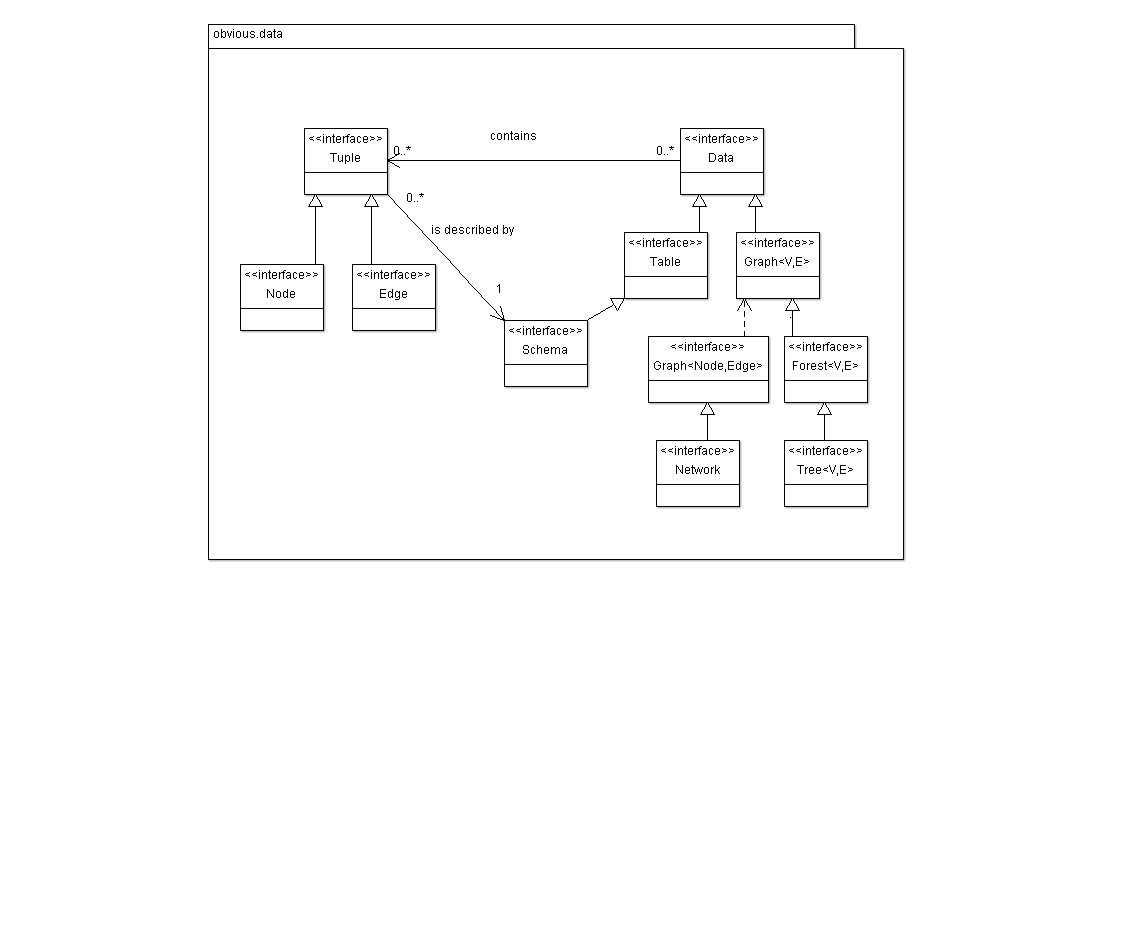
\includegraphics[width=\columnwidth]{figures/obviousdataclass}
\caption{Class diagram of the data model}
\label{fig:datamodel}
\end{figure}

The Obvious data model is centered on the proxy tuple design pattern exposed in \cite{DesignPatternsIV}. Obvious adopts this design pattern to offer high extendability and good usability. Among all the patterns introduced in \cite{DesignPatternsIV}, the proxy tuple pattern enables both as it encompasses graphs in an object-oriented manner - many developers are used to manipulation of \emph{object oriented graphs} - and as it unifies the data model around the same standard structure (tuples and tables). In our data model, tuples are standards elements of all structures: tables are composed of tuples and graphs/trees are implemented as networks i.e. graphs built around two tables one for the nodes and the other for the edges. 

This model is instantiated via factories, that allows cross-toolkit interoperable data structure instantiation. With those factories, it is possible to instantiate tables and networks from a schema or from an existing object from a targeted Obvious implementation (e.g. a Prefuse table or a JUNG graph...). This also provides the possibility to use parameters to provide more arguments used in targeted toolkits. For example, in the Prefuse implementation of Obvious, parameters are used to specify the source and target node columns for a graph in an edge table.

In addition to data access, our data model allows providing 3 optional, interoperable, features: introspection, modifiabilit and notification. Those features are not found in all target toolkit implementations and thus sometimes had to be emulated.
 
\subsection{Introspection}

Introspection means the capability of a program to inspect its own content. In the context of the data model it means mostly that objects expose their own schema explicitely and allow manipulating it as a full fledged object. As an improvement over \cite{DesignPatternsIV}, our data model uses a meta-circular schema design (the schema is itself a table) instead of a column object, that does not exist in Obvious. Schemas have been introduced, first because they are an efficient an elegant mean to gather all \emph{meta-data} for the columns of a table in one unique structure, allowing easy table and network instantiations with a factory. The main use of introspection in a toolkit, though, is to enable generic implementation of a variety of side services as varied as generic persistancy, undo/redo, universal object editors...

\subsection{Modifiability}

Modifiability means that objects in a data model may be edited. This service is not a must-have in an information visualization context, and is actually not even considered in many of the existing toolkits: after all, in many cases, the data may be considered a static object to be analyzed.
Yet new and important usage patterns for combining visualization and data editing have emerged that make this service important~\cite{Discovery3}.

\subsection{Notification}

While most toolkit need to provide a unified notification system to propagate information about changes affecting the data model, it is also not a must-have in the context of an information visualization data-model. Stil,l notification is also an important feature to provide most advanced visualization services. During the development of Obvious implementations, notification systems included in toolkits appeared to be widely different in terms of syntax and functionalities.  That is why the notification system introduced in Obvious is designed to support a large variety of existing notification techniques even those not currently implemented in toolkits. Yet, as in many toolkits \cite{Prefuse,InfoVis,jung2003,Discovery1}, the notification system in Obvious is based on listeners placed on data structures that propagates changes to listening objects. In addition, it supports transaction and batch techniques usually found in database system, as will be seen later.

\subsection{Combining Notification and Modifiability}
\label{sub:combiningnotif}

Combining Notification and Modifiability however raises a challenge. Since one operation can affect a large amout of data, flow of notifications concerning the same action could be generated. This flow can be a problem, since it can increase response time of the application.

\begin{figure}[!ht]

\includegraphics[width=\columnwidth]{figures/notification}
\caption{Sequence diagram for the notification system}
\label{fig:notification}
\end{figure}

Thus, we introduce a method to control the number of emitted notifications: the \emph{beginEdit/endEdit mechanism}. As shown in the figure \ref{fig:notification}, when no mechanism is triggered the change is transmitted to the Listener with \emph{tableChanged} method. This method have several arguments describing the current event (affected Table, rows, columns and operation type). When the \emph{beginEdit} mechanism is enabled, changes are also propagated but different strategies can be applied. It is possible to select a specific strategy with the \emph{mode} parameter. The following strategies have already been developed  in one or more Obvious implementations:

\begin{description}
\item[Lazy strategy] the listener do nothing until it is awake by the endEdit method
\item[Transaction strategy] the listener only commits after the \emph{endEdit} if all data changes occuring between the \emph{beginEdit} and \emph{endEdit} have not violated defined invariants (for example, no null value for a specific field)
\item[Batch strategy] if the batch mode is enabled, all data changes occuring between the \emph{beginEdit} and \emph{endEdit} are placed in a batch, executed after the \emph{endEdit}
\end{description}

\subsection{Data services}

To leverage our core implementation and offer some immediately useful services to Ovious users, we have defined a utility package obviousx, named in the same way as javax. This package provides different kinds of utility classes for the Obvious data model. First, we have defined in obviousx, reader and writer interfaces allowing the creation of gateways between the Obvious data model and common data formats such as CSV and GraphML. It provides software developers a standard way to import and export data in Obvious whatever the underlying implementation of the data model is. In addition, for data providers, it simplifies their work because they only have to develop one reader and one writer to be compatible with a large number of toolkits. With the same logic, obviousx furnishes a Java TableModel compatible with the Obvious one: it allows quick creation of a JTable from an Obvious
table. Finally, obviousx also provides wrappers to \emph{transform} obvious data structures into common existing data structures (Prefuse, Ivtk, Jung, more to develop) in order to avoid copying of data when using more than one data model.
